\documentclass[9pt,twocolumn,twoside]{pnas-report}

\templatetype{pnasresearcharticle}

\usepackage{lipsum}

\title{Identifying the Greatest Tour de France Riders Through Network Science}
\author[a,2]{Martin Starič}
\author[a,1]{Matic Stare}
\author[a,b]{Jan } 
\author[b]{Tian }

\affil[a]{University of Ljubljana, Faculty of Computer and Information Science, Ve\v{c}na pot 113, SI-1000 Ljubljana, Slovenia}
%\affil[b]{Other Fine Institutions}

\leadauthor{Martin Starič}
\authordeclaration{All authors contributed equally to this work.}
\correspondingauthor{\textsuperscript{1}To whom correspondence should be addressed. E-mail: ms92204@student.uni-lj.si}

\begin{abstract}
In this project, we constructed a directed multigraph to analyze over a century of Tour de France results (1903–2024).
For each stage, a directed edge was created from every participant to all riders who placed ahead of them, forming a competitive hierarchy for that stage.
By aggregating data from all stages across all editions of the race,
we generated a massive multigraph capturing the cumulative performance dynamics of Tour de France participants.
We then applied the PageRank algorithm to this graph to evaluate and rank riders based on the structure of competitive dominance inherent in their race history.
This approach offers a novel perspective on historical performance, highlighting riders who consistently placed ahead of strong competitors,
regardless of raw wins or podium finishes.
\end{abstract}

\dates{The manuscript was compiled on \today}
\doi{\href{https://ucilnica.fri.uni-lj.si/course/view.php?id=183}{Introduction to Network Analysis} 2024/25}

\begin{document}

\maketitle
\thispagestyle{firststyle}
\ifthenelse{\boolean{shortarticle}}{\ifthenelse{\boolean{singlecolumn}}{\abscontentformatted}{\abscontent}}{}

\dropcap{I}{\bf ntroduction}
Tour de France is the most prestigious cycling event in the world. The multi-stage competition tests the best cyclists across various terrains,
from flat sprints to punishing climbs. While general classification highlights the best overall cyclists, 
it misses certain cyclists who excel in specific domains such as consistent mountain climbers, sprinters and other stage specialists.

This project aims to accumulate all the Tour de France history by constructing a network that captures the relative performance of all riders in each stage from 1903 to 2024.
In this network, each cyclist is connected via directed edges to those who placed ahead of them in a given stage. A single network is then constructed by merging
all the data across all stages and editions; creating a multigraph. To account for different interpretations of performance, we create multiple versions of this multigraph;
each applying a different edge weighting method.

To find the most successful riders we apply the PageRank algorithm to our multigraphs which
enables us to find even the lesser known riders who specialise in certain types of stages.


\begin{figure}[t]\centering%
	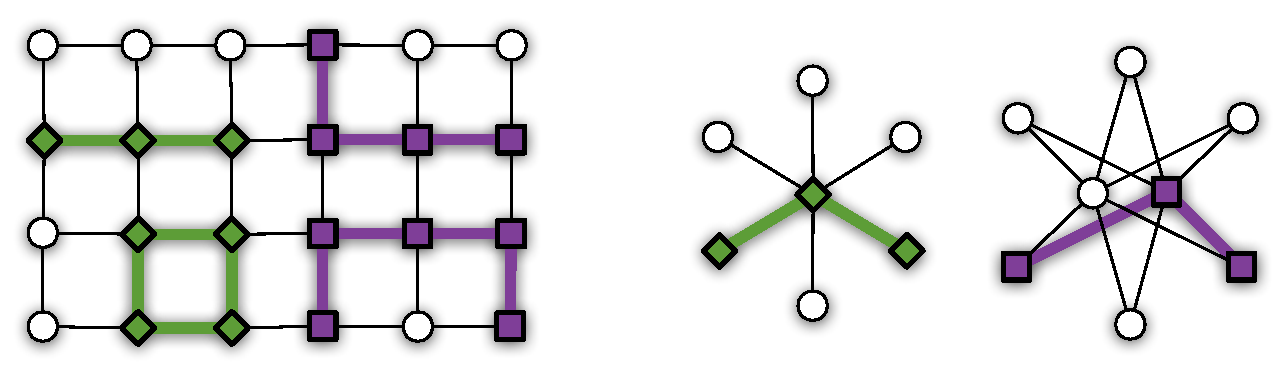
\includegraphics[width=0.9\linewidth]{examples}
	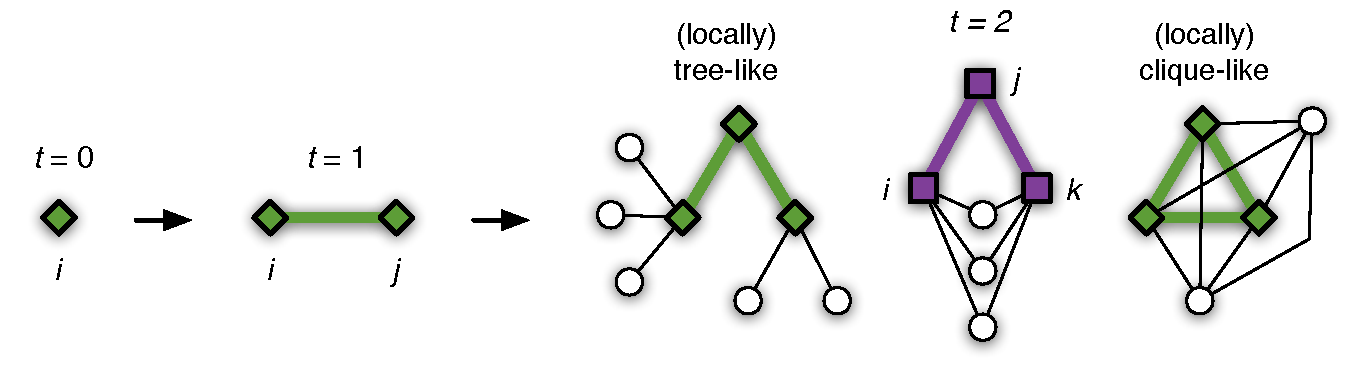
\includegraphics[width=\linewidth]{growth}
	\caption{Mandatory informative illustration highlighting main contributions.~\cite{Sub18a}}
	\label{fig:example}
\end{figure}

\section*{Related work}

{\bf Relevant literature ($\approx 10$ references).}
\lipsum[5-6]

\nocite{Kle00,Bou05,EB07,New08,For10,New12,FH16,PLC17,PDL18,Pei20}

\section*{Results}

{\bf Main results supported by math, plots, tables, diagrams etc.}
\lipsum[1]

\begin{table}[h]\centering%
	\caption{Table describing data or methods.}
	\begin{tabular}{lccccc}\toprule
	    & $n$ & $m$ & $\langle k\rangle$ & $\langle C\rangle$ & $\langle d\rangle$ \\\midrule
	    Fine network & $438\,920$ & $9\,742\,733$ & $44.4$ & $0.37$ & $6.19$ \\
	    Random graph & $438\,920$ & $9\,781\,609$ & $44.6$ & $0.00$ & $4.92$ \\\bottomrule
	\end{tabular}
	\label{tbl:example}
\end{table}

\lipsum[2-3]

\begin{figure}[t]\centering%
	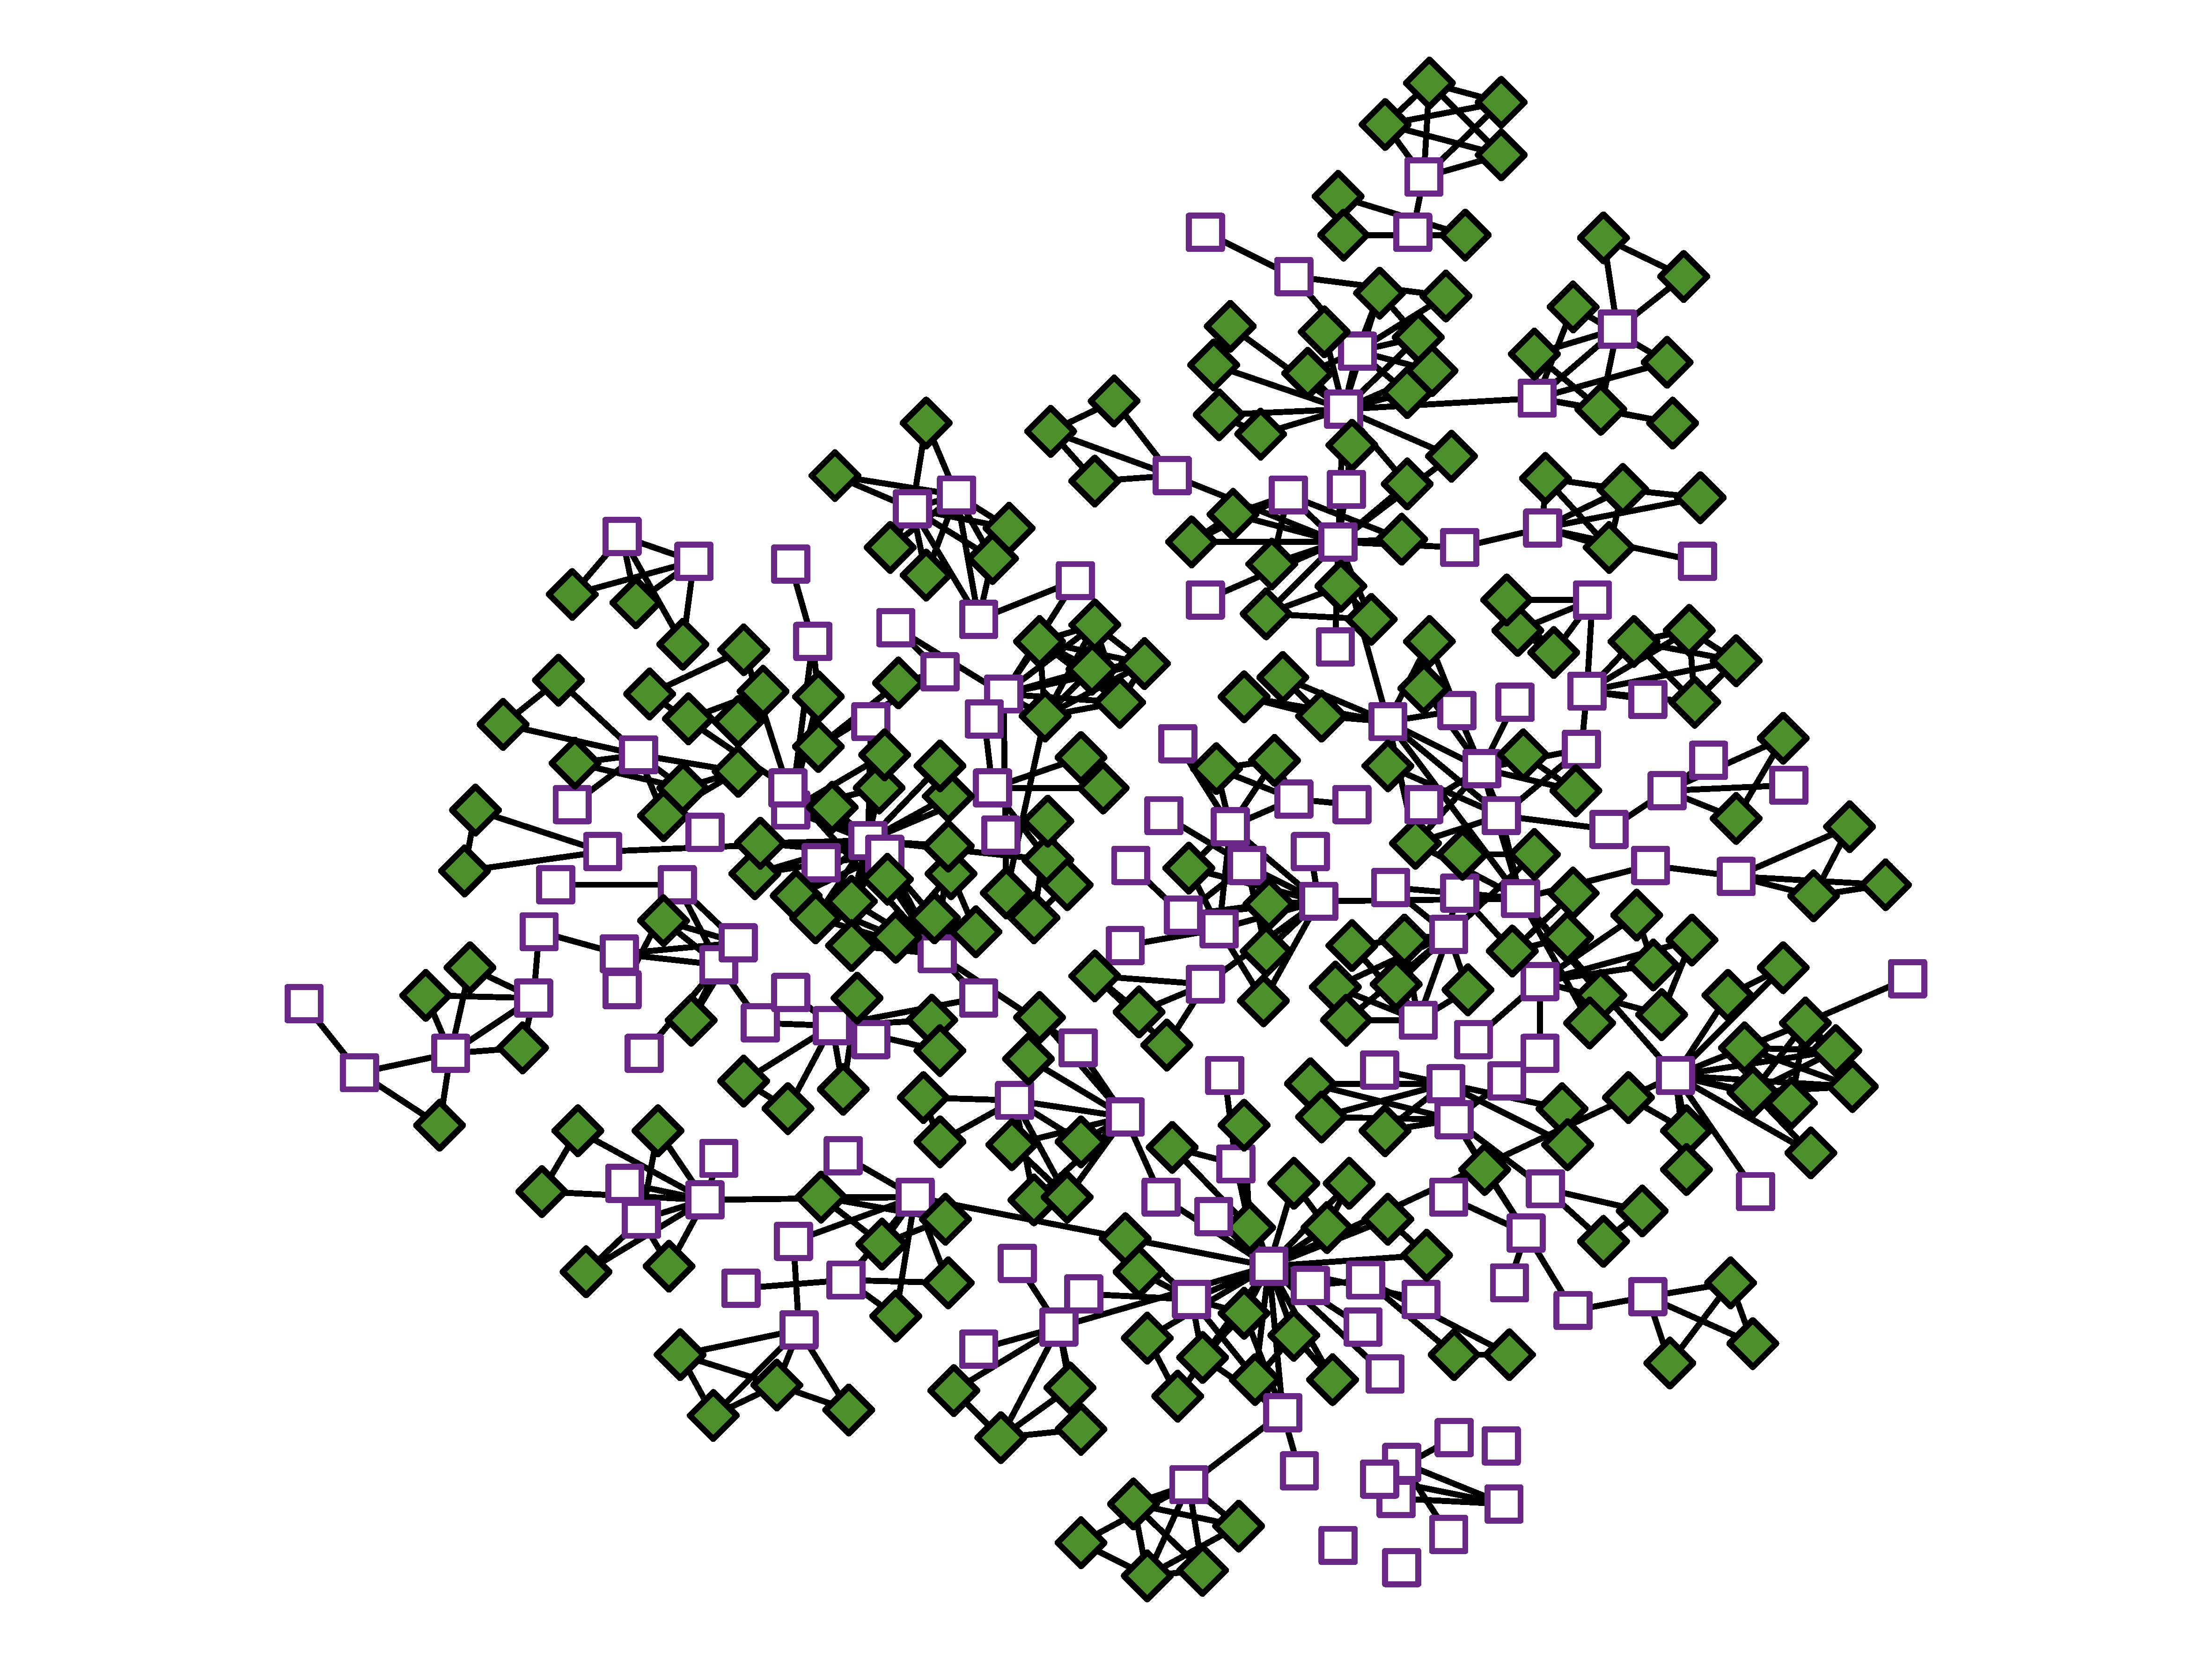
\includegraphics[width=0.49\linewidth]{example1}
	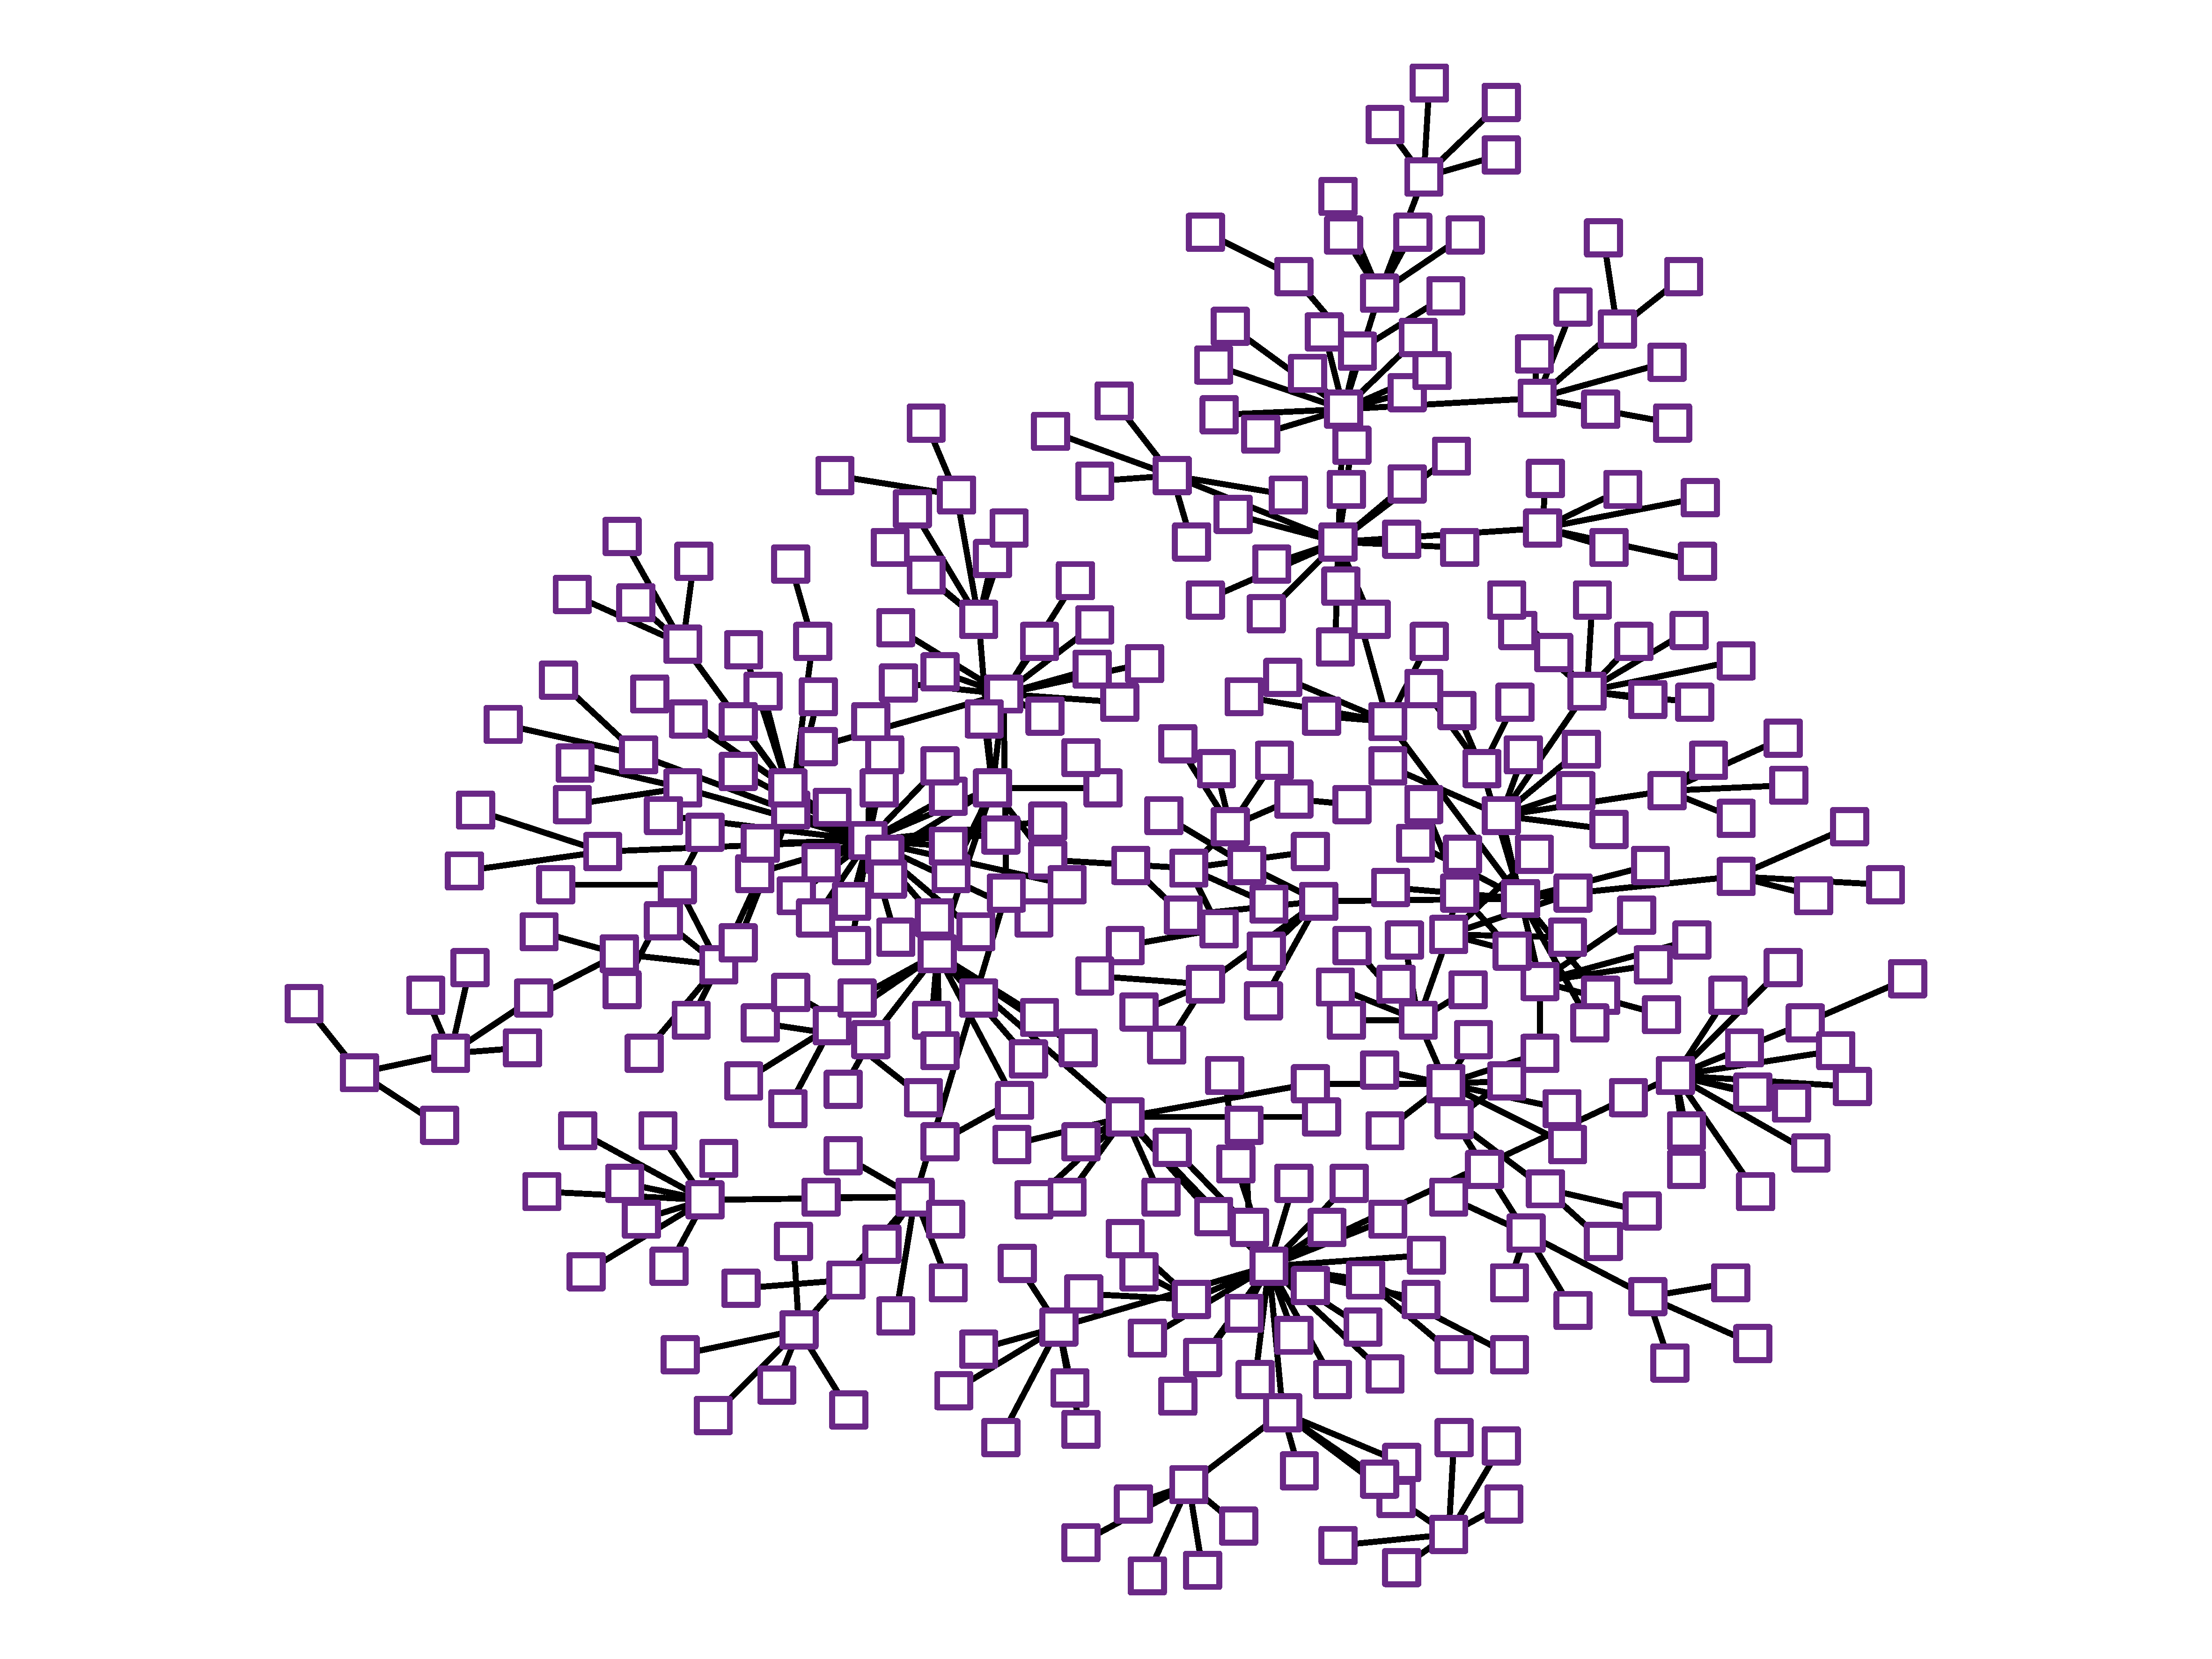
\includegraphics[width=0.49\linewidth]{example2}
	\caption{Figure showing interesting examples.~\cite{Sub18a}}
\end{figure}

\lipsum[4-6]

\begin{figure}[b]\centering%
	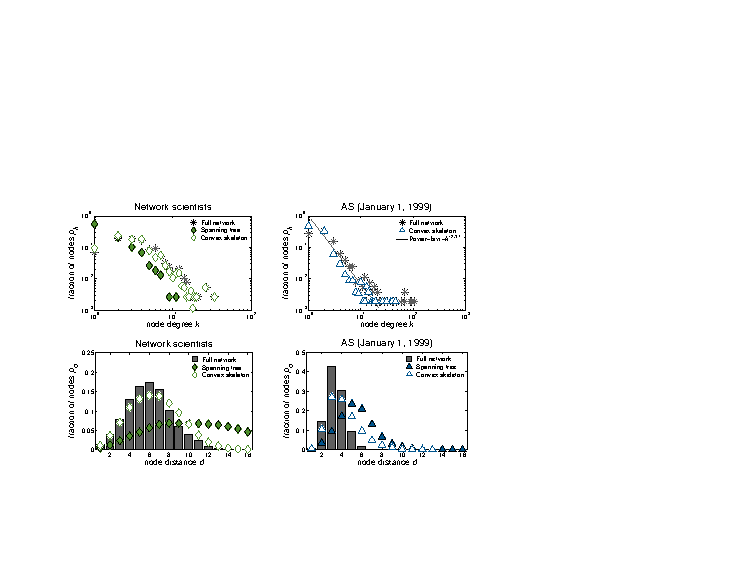
\includegraphics[width=\linewidth]{distributions}
	\caption{Figure showing relevant results.~\cite{Sub18a}}
\end{figure}

\begin{figure}[t]\centering%
	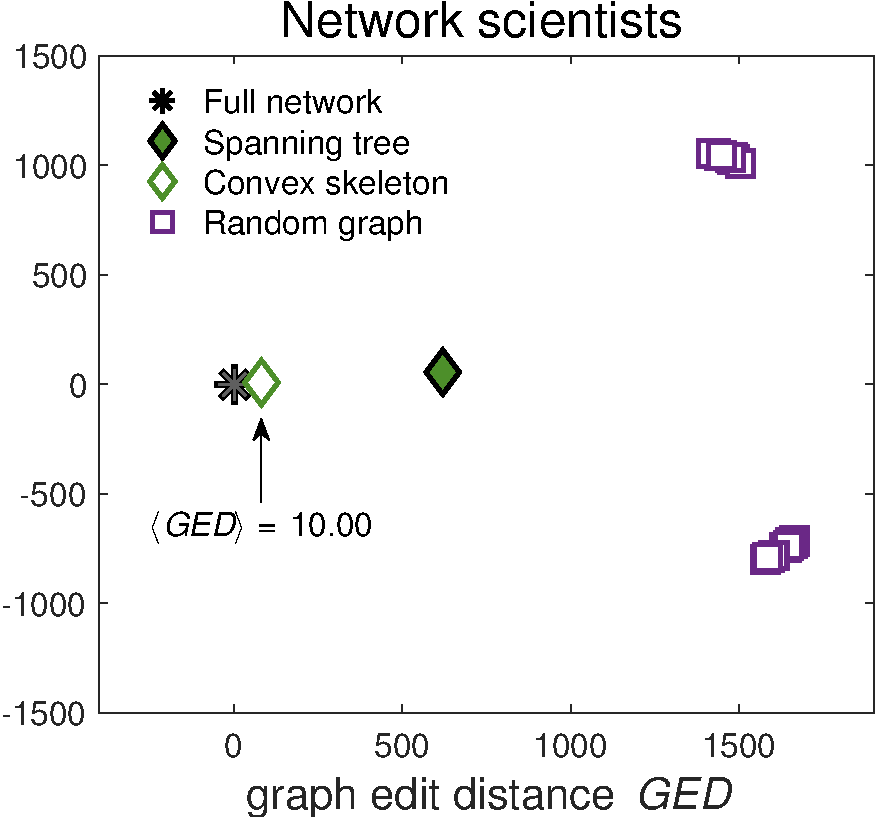
\includegraphics[width=0.45\linewidth]{results1}\hskip12pt
	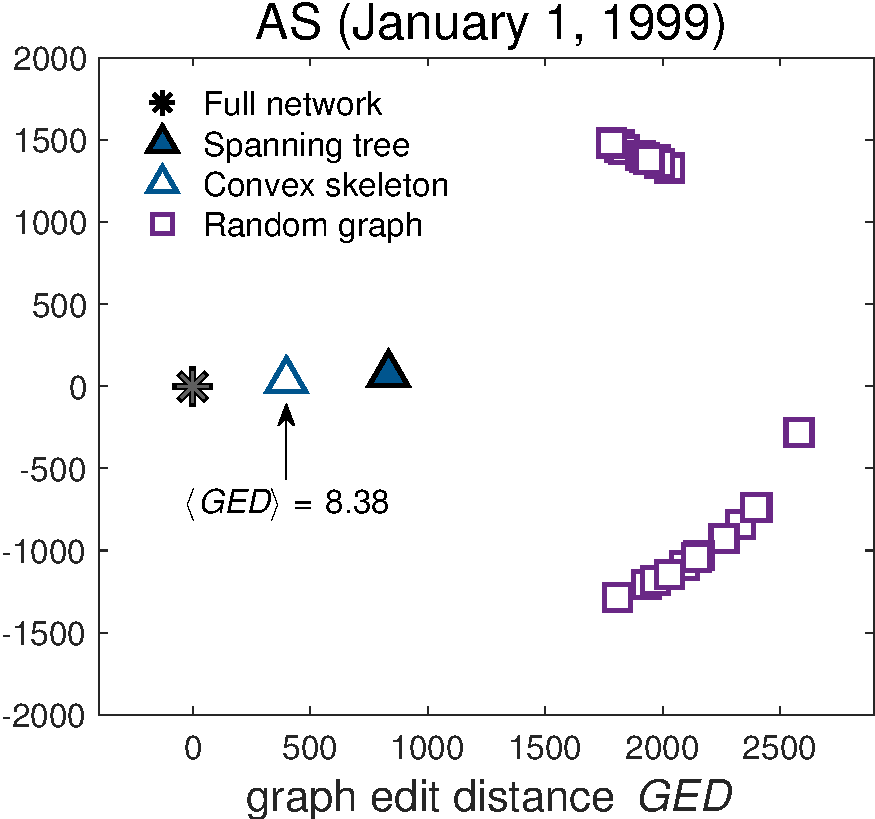
\includegraphics[width=0.45\linewidth]{results2}
	\caption{Another figure with results.~\cite{Sub18a}}
	\label{fig:example}
\end{figure}

\section*{Discussion}

{\bf Summary of results, main contributions, final conclusions, future work etc.}
\lipsum[1-3]

{\small

\section*{Methods}

{\bf Data, methods, algorithms etc.}
\lipsum[1]

\begin{equation}
	\phi_v = \Pr(X_{st}(v) = 1) = \Pr(X_{sv} = 1)\Pr(X_{vt} = 1)
	\label{eq:example}
\end{equation}

\lipsum[2]

\begin{algorithm}[H]
	\begin{algorithmic}[1]
		\Require graph $G$, cutoff $k_{min}$
		\Ensure power-law $\gamma$ 
		\State $s\gets$ $n\gets$ $0$
		\For{nodes $i\in N$} 
			\If {$k_i\geq k_{min}$}
				\State $s\gets$ $s+\ln k_i/(k_{min}-0.5)$
				\State $n\gets$ $n+1$
			\EndIf
		\EndFor
		\State \Return $1+ns^{-1}$
	\end{algorithmic} \vspace{8pt}
\end{algorithm}

\lipsum[3-4]

}

% \acknow{The authors would like to\dots}
% \showacknow{}

\bibliography{bibliography}

\end{document}